% This is LLNCS.DEM the demonstration file of
% the LaTeX macro package from Springer-Verlag
% for Lecture Notes in Computer Science, version 1.1
\documentclass{llncs}
%

\usepackage[utf8]{inputenc} % accents
\usepackage{latexsym}
\usepackage{bbm}              % fontes doubles (pour les ensembles, par ex.)
\usepackage{graphicx}         % pour d'eventuelles figures
\usepackage{epsfig}           % (preferer graphicx, si possible)
\usepackage{amsmath}          % AMSTEX
\usepackage{amsfonts}
\usepackage{fancyhdr}
\usepackage{subfigure}

\usepackage{algorithm}
\usepackage{algorithmic}

\usepackage{hyperref}

\begin{document}

\title{ParKerC: Toolbox for Parallel Kernel Clustering Methods}

\author{Sandrine Mouysset\inst{1} and Ronan Guivarch\inst{2}}

\institute{University of Toulouse, IRIT-UPS, France
\and
University of Toulouse, INP(ENSEEIHT)-IRIT, France}

\maketitle

\begin{abstract}
A large variety of fields such as biology, information retrieval, image
segmentation needs unsupervised methods able to gather data without a priori
information on shapes or locality. By investigating a parallel strategy based
on overlapping domain decomposition, we propose to adapt two kernel
clustering methods respectively based on spectral and density-based properties in order to treat large data sets in fields of pattern
recognition.
\end{abstract}

\section{Introduction}

Many fields from Social Science to Medicine and Biology generate large amount
of data to analyze. Clustering aims at partitioning data sets in clusters in
order to group data points with a similarity measure.  
Kernel clustering methods have become an increasingly popular tool for machine learning \cite{hofmann2008kernel}. These methods rely on the use of positive definite kernel functions which enable them to operate in a high-dimensional feature space and provide, in particular, interesting spectral properties \cite{speC}.  In this paper, we investigate a parallel strategy based
on domain decomposition to treat large data sets for spectral clustering and mean shift \cite{Fukunaga},  two widely used kernel clustering methods.

\section{ParKerC Toolbox}

In this section, we first present the principle of the proposed toolbox. Then
we introduce the kernel clustering methods, their inherent parameters and the
suitability  with a domain decomposition strategy.

\subsection{Principle}
Let consider a data set $S=\{x_i\}_{i=1..n}\in \mathbb{R}^p$. 
The principle of the parallel toolbox is based on domain decomposition with
overlaps. By dividing the data set $S$ in $q$ sub-domains, each processor
applies independently the clustering algorithm on the subsets and provides a
local partition. For each subdomain and each kernel method, the number of
clusters is automatically determined. This heuristic avoids us to fix the
targeted number of clusters.
The final number of clusters $k$ will be provided
after the grouping step. 

The grouping step is dedicated to link the local
partitions from the sub-domains thanks to the overlap  and the
following transitive relation: $\forall x_{i_1}, x_{i_2}, x_{i_3} \in S,$
\vspace{-0.4cm}
\begin{equation}
  \text{if } \ x_{i_1},x_{i_2} \in C^1  \text{ and }  x_{i_2}, x_{i_3} \in C^2 \text{ then } C^1 \cup C^2 = P \text{ and } x_{i_1},x_{i_2}, x_{i_3} \in P \label{reltrans}
\end{equation}

where $C^1$ and $C^2$ two distinct clusters and $P$ a
larger cluster which includes both $C^1$ and $C^2$.  By applying this
transitive relation (\ref{reltrans})  on the overlap, the
connection between subsets of data is established and provides a global
partition.

We can implement this algorithm using a Master-Slave paradigm as summarized in
%We can summarize this Master-Slave implementation with Algorithm
algorithms \ref{algo-master} and \ref{algo-slave}.

\vspace{-0.5cm}

\begin{algorithm}
\caption{Parallel Algorithm: Master}
\label{algo-master}
\begin{algorithmic}[1]
%\begin{algorithm}
  \STATE Pre-processing step\\
        1.1 Read the global data and the parameters\\
        1.2 Split the data into $q$ subsets\\
        1.3 \begin{tabular}[t]{l}
            Compute the affinity parameter $\delta$ with the formula given 
            in paper \ref{delta}; \\
            the bandwidth of the overlapping is fixed to
            $c \times \delta$  with $c \in \mathbb{N}$.
            \end{tabular}
  \STATE Send $\delta$ and the data subsets to the slaves
         %(\textsc{Mpi\_Send})
  \STATE Perform the Clustering Algorithm on its subset\\
  \STATE Receive the local partitions and the number of clusters from each
         slave %(\textsc{Mpi\_Recv})
  \STATE Grouping Step\\
         5.1 Gather the local partitions in a global
         partition with the transitive relation~(\ref{reltrans})\\
         5.2 Output a partition of the whole data
         set $S$ and the final number of clusters $k$
\end{algorithmic}
\end{algorithm}

\vspace{-1.2cm}

\begin{algorithm}[!h]
\caption{Parallel Algorithm: Slave}
\label{algo-slave}
\begin{algorithmic}[1]
%\begin{algorithm}
  \STATE Receive $\delta$  and its data subset from the Master
  \STATE Perform the Clustering Algorithm on its subset
  \STATE Send its local partition and its number of clusters to the Master
\end{algorithmic}
\end{algorithm}

\vspace{-1cm}

\subsubsection{Overlapping bandwidth}

The idea is to consider an uniform distribution where data points are
separated by the same distance each other. To define this distance, we
consider both the dimension of the problem as well as the density of points in
the given $p$-th dimensional data set.  In fact, the data set $S$ is included
in a $p$-dimensional box bounded by $\rho_d$ the largest distance between
pairs of points in each dimension $d$ of $S$: 
$ \rho_d=\max_{1\leq i,j \leq n}  |x_{id} - x_{jd}|,\ \forall d\in \{1,..,p\}$. \\ So the uniform distance  noted $\delta$ could be defined as follows:

\begin{equation}
  \delta = \left(\frac{\prod_{i=1}^p{\rho_i}}{n}\right)^{\frac{1}{p}}. \label{delta}
\end{equation}

\noindent From this distance, the ovelapping bandwidth is set as a multiple of $\delta$.

In the following, we present two kernel clustering methods, the spectral
clustering and  the mean shift, and how to tune inherent parameters of both
methods.  The first method based on eigen-decomposition of kernel affinity
matrix is used in pattern recognition or image segmentation  to cluster
non-convex domains without a priori on the shapes. The second method relies on
a non-parametric estimator of density gradient for locating the maxima of the
density function called mode.

\subsection{Spectral clustering}

Spectral clustering uses eigenvectors of a matrix, called Gaussian affinity
matrix, in order to define a low-dimensional space in which data points can be
clustered.

\subsubsection{Algorithm}

Assume that the number $k$ of targeted clusters is known (we will see how to automatically determine it). First, the spectral
clustering consists in constructing the affinity matrix based on the Gaussian
affinity measure between points of the dataset $S$.  After a normalization
step, the $k$ largest eigenvectors are extracted. So every data point $x_i$ is
plotted in a spectral embedding space of $\mathbb{R}^k$ and the clustering is
made in this space by applying $K-means$ method. Finally, thanks to an
equivalence relation, the final partition of data set is defined from the
clustering in the embedded space. Algorithm \ref{algoSC} presents the
different steps of spectral clustering.

\vspace{-0.5cm}
\begin{algorithm}
\caption{Spectral Clustering Algorithm}
%\begin{algorithmic}[1]
%\begin{algorithm}
Input: data set $S$, number of clusters $k$
\begin{enumerate}
  \item Form the affinity matrix $A\in\mathbb{R}^{n\times n}$ defined by:
    \begin{equation}
      A_{ij}=\begin{cases}
        \exp\left(-\frac{\left\|x_i-x_j\right\|^2}{(\sigma/2)^2}\right) \text{\  if $i\neq j$,}\\ \label{defaff}
        0 \ \text{otherwise,}
      \end{cases}
    \end{equation}
  \item Construct the normalized matrix: $L=D^{-1/2}AD^{-1/2}$ with $D_{i,i}=\sum_{j=1}^n A_{ij}$,
  \item Assemble the matrix $X=[X_1X_2..X_k]\in \mathbb{R}^{n\times k}$ by stacking the eigenvectors associated with the {$k$} largest eigenvalues of $L$,
  \item Form the matrix Y by normalizing each row in the $n \times k$ matrix X,
  \item Treat each row of Y as a point in $\mathbb{R}^{k}$, and group them in $k$ clusters via the {\it K-means} method,
  \item Assign the original point $x_i$ to cluster $j$ when row $i$ of matrix Y belongs to cluster~$j$. 
\end{enumerate}
\label{algoSC}
%\end{algorithmic}
\end{algorithm}

\vspace{-1.0cm}

\subsubsection{Justification}

From the definitions of  both the Gaussian affinity $A_{ij}$ between two data
points $x_i$ and $x_j$ and the Heat kernel $K_t(x)=(4\pi
t)^{-\frac{p}{2}}\exp\left(-{\|x\|^2}/{4t}\right)$ in free space
$\mathbb{R}^*_+ \times \mathbb{R}^p$, we can interpret the gaussian affinity
matrix as discretization of heat kernel by the following equation:

\begin{equation}
  A_{ij}=(2\pi \sigma^2)^{\frac{p}{2}} K_t\left({\sigma^2}/{2},x_i-x_j\right). \label{lien}
\end{equation}

So, we can prove that eigenfunctions for bounded and free space Heat equation
are asymptotically close \cite{mouysset2,mouysset2014spectral}. With Finite
Elements theory, we can also prove that the difference between eigenvectors of
$A$ and discretized eigenfunctions of $K_t$ is of an order of the distance
between points include inside the same cluster. This means that applying
spectral clustering into subdomains resumes in restricting the support of
these $L^2$ eigenfunctions which have a geometrical property: their supports
are included in only one connected component.

Thus, the overlapping domain decomposition does not alter the
global partition because the eigenvectors carry the geometrical property and
so, the clustering property.

\subsubsection{Tuning parameters}

Spectral clustering depends on two parameters: the Gaussian affinity parameter
$\sigma$ and the number of clusters $k$.  The \textit{Gaussian affinity
matrix} (\ref{defaff}) is widely used and depends on a free parameter
$\sigma$. It is known that this parameter affects the results in spectral
clustering and spectral embedding.  From the definition of $\delta$ defined by
(\ref{delta}) in which we consider the case of an uniform distribution in the
sense that all pair of points are separated by the same distance $\delta$ in
the box of edge size $D_{max}$,  we can state that clusters may exist if there
are points that are at a distance no more than a fraction of $\delta$. \\
\noindent The \textit{number of clusters} $k$  is defined from a measure based
on the ratio of the Frobenius norms of the affinity measure between distincts
clusters and within clusters \cite{mouysset3}. The value of $k$ that minimizes
this ratio becomes the number of clusters.


\subsection{Mean shift}

Introduced by Fukunaga and Hostetler \cite{Fukunaga}, mean shift method considers the
points in the feature space as a probability density function. Dense regions
in feature space corresponds to local maxima (or mode). The clusters are then
associated with the modes.

\subsubsection{Algorithm}
Mean shift associates each data point in $\mathbb{R}^p$ with the
nearby peak of the dataset's probability density function. For each data
point, mean shift defines a window around it and computes the mean of the data
points which belong to this window. Then it shifts the center of the window to
the mean and repeats the algorithm till it converges. In other words, the
window shifts to a more denser region of the dataset.

\vspace{-0.5cm}

\begin{algorithm}
\caption{Mean shift Algorithm}
Input: data set $S$, bandwidth $h$\\
 For each data point $x_i\in S$, 
 \begin{enumerate}
   \item Compute mean shift vector $m(x_i)^t$ 
   \item Move the density estimation window to $m(x_i)^t$
   \item repeat till convergence i.e $\|m(x_i)^{(t+1)}-m(x_i)^t\|\leq threshold$
 \end{enumerate}
\end{algorithm}

\vspace{-1.0cm}

\subsubsection{Justification}

Mean shift relies on kernel density estimation.  Kernel density estimation
\cite{Rosenblatt} (also called the Parzen window technique \cite{Parzen}) is
the most popular non parametric density estimation method. Given a kernel $K$,
a bandwith parameter $h$, kernel density estimator for a given set of $n$
$p$-dimensional points is:

\begin{equation}
  f(x)=\frac{1}{nh^p}\sum_{i=1}^n K\left(\frac{x-x_i}{h}\right)
\end{equation}

Mean shift is based on Gradient ascent on the density contour \cite{Comaniciu1999}. So, for each
data point, we perform gradient ascent on the local estimated density until
convergence. So:

\begin{equation}
  \nabla f(x)=\frac{1}{nh^p}\sum_{i=1}^n K'\left(\frac{x-x_i}{h}\right)
\end{equation}

where $K'(x)$ is the derivative of $K(x)$.  The stationary points obtained via
gradient ascent represent the modes of the density function. All points
associated with the same stationary point belong to the same cluster. By
assuming that $g(x)=-K'(x)$, the following quantity $m(x)$, called mean shift,
is computed as follows:

\begin{equation}
m(x)=\frac{\sum_{i=1}^n g\left(\frac{x-x_i}{h}\right)x_i}{\sum_{i=1}^n g\left(\frac{x-x_i}{h}\right)}-x
\end{equation}

With this strategy of searching the maximum of local density,  this method
does not require to fix the number of clusters. 

This implies that mean shift
can be runned in subsets of $S$ and if a cluster relies on several subdomains
then the transitive relation (\ref{reltrans}) will merge the subclusters.

\subsubsection{Tuning parameters}

As said in the previous section, the number of clusters is automatically
defined.  But mean shift is sensitive to the selection of bandwidth $h$.  A
small $h$ can slow down the convergence whereas a larger one can speed up the
convergence and merge two modes. We can define it automatically by considering
the bandwidth $h$ as a multiple of the uniform distance $\delta$ defined
by~(\ref{delta}).

\section{Implementation and results}

The code of the ParKerC toolbox is written in FORTRAN 90 using MPI library to
handle the communication between processors.

\subsection{Application to clustering datasets}

We present in this Fig.\ref{datasets} some results on four different datasets from a clustering \href{https://cs.joensuu.fi/sipu/datasets/}{benchmark} to validate our parallel approach: 

$$
\begin{array}{|c|c|c|c|c|}
  \hline
  &  \mbox{unbalance} & \mbox{spiral} & \mbox{Compound3} & \mbox{jain}\\
  \hline
  \mbox{Size} & 6500 & 312 & 219 & 373\\
  \hline
  \mbox{Nb Clusters} & 8 & 3 & 3 & 2\\
  \hline
\end{array}
$$

Each problem is solved by using spectral clustering or mean shift methods, in
sequential ($1\times1$) and in parallel ($2\times2$ square-partitioning).
We tuned the parameters as explained in the theoretical sections: $\delta$
is computed; we used it to control the spectral clustering, 
to define the bandwidth for the mean shift ($C \times \delta$) and
the overlapping bandwidth ($2\times \delta$) for domain partitioning.

\begin{figure}[!h]
  \begin{center}
    %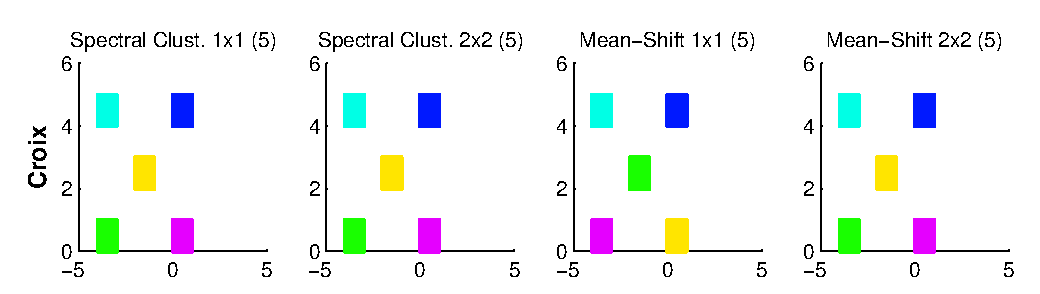
\includegraphics[width=\linewidth]{Croix}
    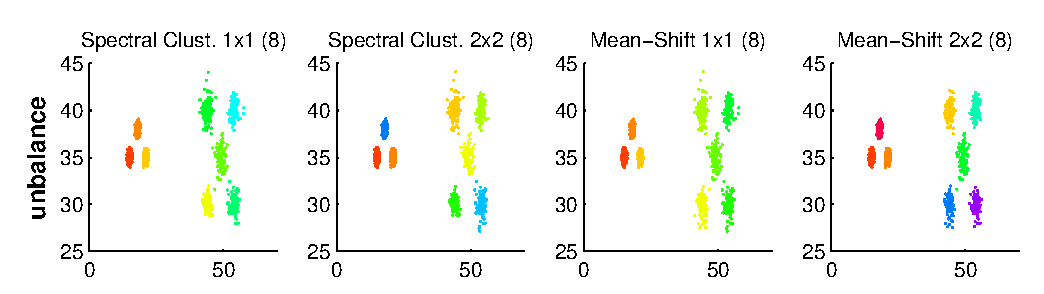
\includegraphics[width=\linewidth]{unbalance}
    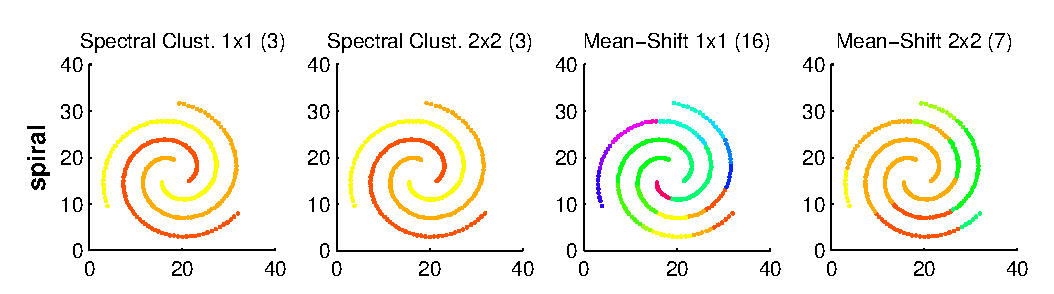
\includegraphics[width=\linewidth]{spiral}
    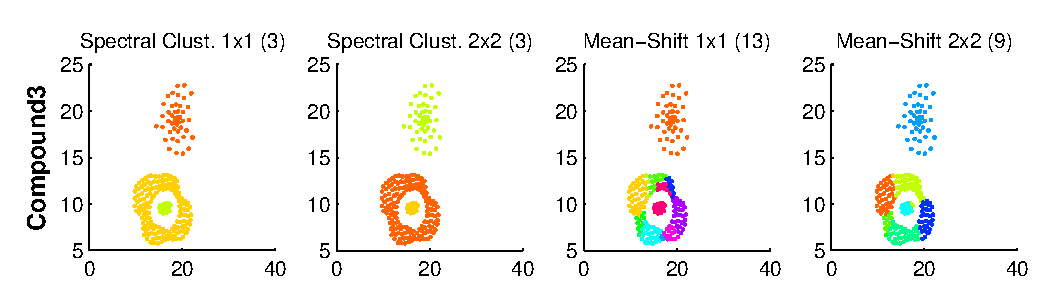
\includegraphics[width=\linewidth]{Compound3}
    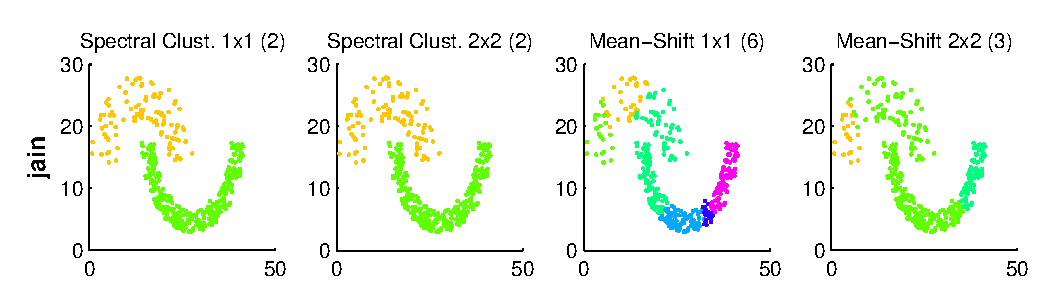
\includegraphics[width=\linewidth]{jain}
  \end{center}
  \caption{Examples of dataset segmentation}
  \label{datasets}
 \end{figure}


We can notice that spectral clustering gives expected results for all
problems both in sequential and in parallel (the number of exhibited clusters
are between parenthesis). In contrary, mean shift have good
results when the clusters are convex but poor ones with non-convex clusters;
we tried different values of $C$ and present the less worse results.
With no post-treatment (for instance, merging using transitivity), its results
are not exploitable.

However for the examples where mean shift has a good behavior, it is much
faster than spectral clustering.
%(when we don't use sparsification \cite{vec2012}).

\subsection{Application to image segmentation}

For image segmentation, the domain decomposition is applied geometrically on
the image and also on the brightness distribution (or color
levels).
Thus, the kernel function is applied on geometrical and brightness/color data. The kernel function $K$ at a pixel $x$ will be decomposed according to the spatial and color vectors as:  
\begin{equation}
K_{h_r,h_s}(x)=K\left(\frac{x^s}{h_s}\right)K\left(\frac{x^r}{h_r}\right)
\end{equation}
where $x^s\in \mathbb{R}^2$ is the spatial vector of the pixel $x$ and $x^r \in \mathbb{R}^3$ is the 3D color level vector of $x$ and $h_s$ and $h_r$ are respectively the spatial and color parameters.
We apply in parallel both spectral clustering and mean shift on a geometrical
picture as shown in Fig.\ref{res-img} and Fig.\ref{Taeuber} (painting inspired from
Swiss artist, Sophie Taeuber-Arp).

\begin{figure}
  \begin{center}
    \subfigure[original image]{\includegraphics[width=0.3\linewidth]{croissants-original}}
    \subfigure[mean shift ($5 \times 4$) ]{\includegraphics[width=0.3\linewidth]{croissants-ms}}
    %\{14~clusters\}
    \subfigure[spectral clust. ($5 \times 4$) ]{\includegraphics[width=0.3\linewidth]{croissants-sc}}
   % \{91~clusters\}
  \end{center}
  \caption{Results of parallel clustering methods on an image ($275 \times
  194$)}
  \label{res-img}
\end{figure}

\begin{figure}
  \begin{center}
    \subfigure[original
    painting]{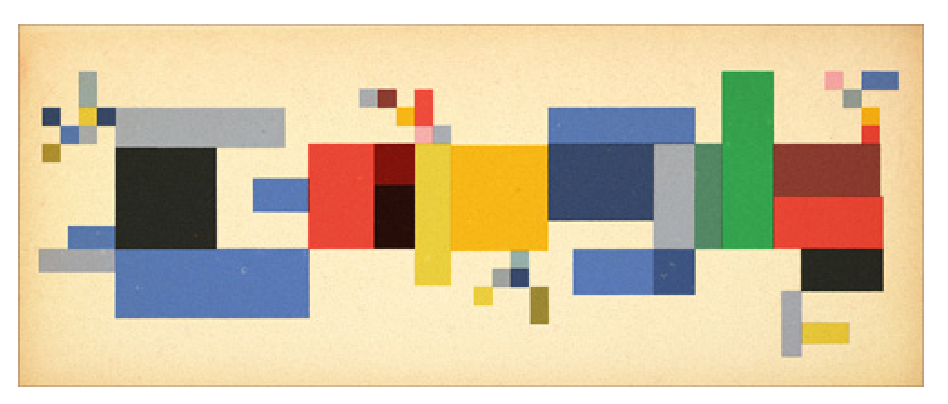
\includegraphics[width=0.3\linewidth]{Taeuber-original}}
    \subfigure[mean shift ($5 \times 4$) ]{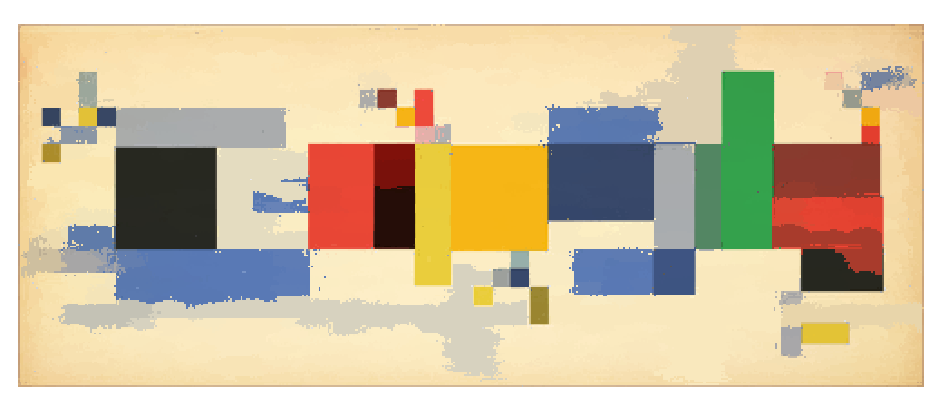
\includegraphics[width=0.3\linewidth]{Taeuber-ms}}
   %\{1605~clusters\}
    \subfigure[spectral clust. ($5 \times 4$) ]{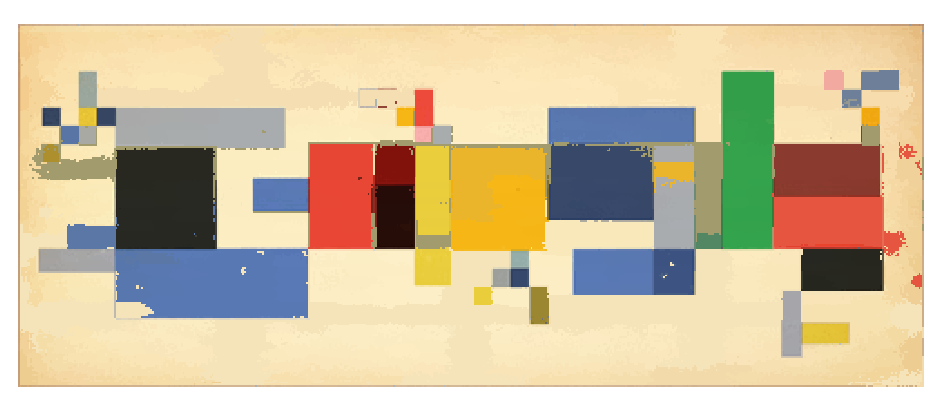
\includegraphics[width=0.3\linewidth]{Taeuber-sc}}
  \end{center}%\{1400~clusters\}
  \caption{Results of parallel clustering methods on a painting ($500 \times
  200$)}
  \label{Taeuber}
\end{figure}


\section{Conclusion and perspectives}

We have validated the two parallel methods, both with small datasets and an image.
We will continue our tests on larger problems to fully validate our FORTRAN
code. These kernel methods offer different clustering analysis. Spectral clustering, based on connected components,  can partition clusters with uniform distribution and circular shapes. Mean shift, relied on a density-based approach, can separate clusters even when they are connected by few points. 


%On the theoretical part, we want to investigate some other expressions of
%$\delta$ to better approximate the data distribution (for instance replace the
%euclidian distance by $L1-$norm). We also plan  to investigate different
%kernel functions.

Our spectral clustering method on a sub-domain uses sequential version of
algebra linear kernels (LAPACK or ARPACK). Chen et al \cite{Chen10} proposed a parallel version of the spectral clustering method that can be used on one subdomain. In the same way, we can modify the mean shift on each subdomain by the fully parallel mean shift of  Varga et al \cite{varga2011high}. Thus, for both
spectral clustering and mean shift, we can imagine a two-stage parallel
implementation: sub-domain decomposition and then a parallel solution on each
sub-domain. 
%\vspace*{-0.5cm}

%\newpage
\begin{thebibliography}{5}
{
\bibitem{hofmann2008kernel}
{Hofmann, T. and Sch{\"o}lkopf, B. and Smola, A. J},
{Kernel methods in machine learning},
\emph{The annals of statistics},
{1171--1220},
{2008}.

\bibitem{speC}
Ng, A. Y. and Jordan, M. I. and Weiss, Y.,
On spectral clustering: analysis and an algorithm,
\emph{Proc.Adv.Neural Info.Processing Systems},
2002.

\bibitem{mouysset2}
Mouysset, S. and Noailles, J. and Ruiz, D.,
On an interpretation of Spectral Clustering via Heat equation and Finite
Elements theory,
\emph{International Conference on Data Mining and Knowledge Engineering},
2010.

\bibitem{mouysset3}
Mouysset, S. and Noailles, J., Ruiz, D. and Guivarch, R.,
On a strategy for Spectral Clustering with parallel computation,
\emph{High Performance Computing for Computational Science: 9th International Conference},
2010.

\bibitem{mouysset2014spectral}
Mouysset, S. and Noailles, J. and Ruiz, D. and Tauber, C.,
{Spectral Clustering: interpretation and Gaussian parameter},
\emph{Data Analysis, Machine Learning and Knowledge Discovery},
153--162, 2014.

\bibitem{Fukunaga}
Fukunaga K. and Hostetler L.D., 
{The Estimation of the Gradient of a Density Function, with Applications in Pattern Recognition},
\emph{IEEE Transactions on Information Theory},
vol 21, 32--40, 1975.

\bibitem{Comaniciu1999}
Comaniciu, D. and Meer, P.,
Mean shift analysis and applications,
\emph{Proceedings of the 7th IEEE International Conference on Computer Vision},
1197--1203, 1999.

\bibitem{Rosenblatt}
Rosenblatt, M.,
Remarks on some nonparametric estimates of a density function,
\emph{The Annals of Mathematical Statistics},
27, 3, 832--837, 1956.

\bibitem{Parzen}
Parzen, E.,
On estimation of a probability density function and mode,
\emph{The annals of mathematical statistics},
1065--1076, 1962.

%\bibitem{vec2012}
%Mouysset, S. and Guivarch, R.,
%Sparsification of Parallel Spectral Clustering,
%\emph{High Performance Computing for Computational Science, Kobe},
%{249--260}, 2012.


\bibitem{Chen10}
Chen, W-Y. and Yangqiu, S. and Bai H. and Lin C-J. and Chang E. Y.,
Parallel Spectral Clustering in Distributed Systems,
\emph{IEEE Transactions on Pattern Analysis and Machine Intelligence},
2010.

\bibitem{varga2011high}
Varga, B. and Karacs, K.,
High-resolution image segmentation using fully parallel mean shift,
\emph{EURASIP Journal on Advances in Signal Processing},
{1--17}, 2011.

}
\end{thebibliography}

\end{document}
